\documentclass[10pt, a4paper]{amsart}

\usepackage[]{graphicx}
\usepackage[]{hyperref}
\usepackage[]{physics}
\usepackage[]{listings}
\usepackage[utf8]{inputenc}
\usepackage[toc,page]{appendix}

\lstset{
	frame = single,
	language = C++,
	showstringspaces = false,
	tabsize = 2,
	otherkeywords = {self},
	keywordstyle = \color{blue},
	identifierstyle=\color{deepgreen},
 	stringstyle=\color{orange},
 	backgroundcolor=\color{mygray}
}

\title[Schrödinger's Equation in 3D]{Schrödinger's Equation in a Three-Dimensional Harmonic Oscillator Well \\
  \hrulefill\small{ FYS3150: Computational Physics }\hrulefill}
  
\author[Winther-Larsen \& Svalheim]{Sebastian G. Winther-Larsen \\ 
Trygve L. Svalheim \\
\href{https://github.com/gregwinther/FYS3150/}{\texttt{github.com/gregwinther}}}
  
\begin{document}

\begin{titlepage}
\begin{abstract}
In this project we have solved the three-dimensional Schrödinger equation for two particles with and without a repulsive Coulomb potential in an harmonic oscillator well. By discretizing the equation for one and later two electrons we could solve it numerically as an eigenvalue problem using the Jacobi method. By implementing the algorithm we observe that the numerical solution coincides well with the analytical prediction. Furthermore, the only difference between the cases with and without Coulomb repulsion is the potential term, hence we can conclude that our algorithm can be modified for any potential. 
\end{abstract}
\maketitle
\tableofcontents
\end{titlepage}

\section{Introduction}

The aim of this study is to solve Schrödinger's equation for two electrons in a three-dimensional  harmonic oscillator well with and without repulsive Coulomb interaction. The equation is reformulated to a discretized in order to be represented as a matrix eigenvalue problem that can be solved with Jacobi's method. Third, a brief discussion of how to implement the algorithm. To keep this article brief and to the point we have forgone to include any code snippets, but everything can be found at the github address stated above. Fourth and lastly, we present the results and give some concluding remarks.

\section{Theory}
We assume that electrons confined in a small area move in a three-dimensional harmonic oscillator potential and repel each other via the static Coulomb interaction. To simplify the problem, spherical symmetry is assumed. First, we give a brief theoretic outline of the radial Scchrödinger equation in order to av a theoretical base for the study. Second, we give a thorough description of how an algorithm for an eigenvalue problem must function. Third, we 

\subsection{A single electron}
The radial part of Schrödinger's equation for a single electron reads
\begin{equation}
\label{eq:schr1}
-\frac{\hbar^2}{2m}\left(\frac{1}{r^2}\frac{d}{dr}r^2\frac{d}{dr}-\frac{l(l+1)}{r^2} \right)R(r) + V(r)R(r) = ER(r)
\end{equation}
where $V(r)$ is the harmonic oscillator potential\footnote{One can in theory insert any potential into the Schrödinger equation, but in this case the harmonic oscillator potential is employed.}, $V(r)=\frac{1}{2}kr^2$ where $k=m\omega^2$, and consequently $E$ is the energy of the harmonic oscillator in three dimensions. The angular frequency of the oscillator is given by $\omega$ and is related to the energy of the system as follows
\begin{equation}
E_{nl}=\hbar\omega\left(2n + l  + \frac{3}{2} \right), \quad n,l \in \mathbb{N} 
\end{equation}
However, we will consider cases with zero angular momentum only ($l=0$). Moreover, by a somewhat lengthy substitutive exercise will culminate in a rewriting of Schrödinger's equation in \ref{eq:schr1} to a dimensionless form
\begin{equation}
\label{eq:schr2}
-\frac{d^2}{d\rho^2}u(\rho) + \rho^2u(\rho) = \lambda u(\rho)
\end{equation}
where $u(r) = R(r)/r$ and $\rho = r/\alpha$ is a dimensionless parameter for length. The constant $\alpha$ is $\alpha = \sqrt{\hbar^2/mk}$ and the energy parameter (eigenvalues) are $\lambda = 2m\alpha^2E/\hbar^2$. The three first eigenvalues will be $\lambda_0= 3$, $\lambda_1 = 7$ and $\lambda_0=11$.

The second derivative in equation \ref{eq:schr2} will be approximated by the well-known central finite difference method for the second derivative,
\begin{equation}
\frac{du^2}{d\rho^2}=\frac{u(\rho+h)-2u(\rho)+u(\rho-h)}{h^2}+\mathcal{O}(h^2)
\end{equation}
where $h = (\rho_N-\rho_0)/h$ is the step size. By denoting $u(\rho_0+ih)$ by $u_i$, equation \ref{eq:schr2} can be further rewritten to
\begin{align}
-\frac{1}{h^2}u_{i-1}+\left(\frac{2}{h^2} + \rho_i^2 \right)u_i-\frac{1}{h^2}u_{i+1}=\lambda u_i \label{eq:schr3}\\
A\vb{u} = \lambda \vb{u} \label{eq:mat1}
\end{align} 
where the matrix in \ref{eq:mat1} is
\begin{equation}
\begin{bmatrix}
\frac{1}{h^2} + \rho_i^2 & -\frac{1}{h^2} & 0 & 0 & 0 & \dots & 0 \\
-\frac{1}{h^2} & \frac{1}{h^2} + \rho_i^2 & -\frac{1}{h^2} & 0 & 0 & \dots & 0 \\
0 & -\frac{1}{h^2} & \frac{1}{h^2} + \rho_i^2 & -\frac{1}{h^2} & 0 & \dots & 0  \\
\vdots & \vdots & \vdots &\ddots & \ddots & \ddots & \vdots \\
0 & 0 & 0 & \dots &  -\frac{1}{h^2} & \frac{1}{h^2} + \rho_i^2 & -\frac{1}{h^2} \\
0 & 0 & 0 & 0 & \dots & -\frac{1}{h^2} & \frac{1}{h^2} + \rho_i^2 
\end{bmatrix}
\end{equation}

By finding the eigenvectors, or the energies, corresponding to the eigenvalues $\lambda_i$  equation \ref{eq:schr3} above, one has found the wave function that describe the behavior of the electron for a particular state $i$. It is of interest to also state the exact, analytical wave function for the three lowest states, because the Schrödinger equation in general is only analytically solvable for a select few potentials, and the harmonic oscillator potential is amongst these. The general form of these radial wave function solutions is 
\begin{equation}
\label{eq:radialschr1}
R_{n,l=0}(r)=N_ne^{-\frac{m\omega}{2\hbar}r^2}\sqrt{L_n}\left(-\frac{m\omega}{2\hbar} r^2 \right)
\end{equation}
where $L_n$ refers to a particular Laguerre polynomial. More on the Laguerre polynomials can be found in appendix \ref{app:laguerre}. Reevaluating this function for the three lowest energy states and normalizing yields the following equations
\begin{align}
\abs{u_0(\rho)}^2 &= \frac{4}{\sqrt{\pi}}\rho^2e^{-\rho^2} \\
\abs{u_1(\rho)}^2 &= \frac{8}{3\sqrt{\pi}}\rho^2\left( \frac{3}{2}-\rho^2 \right)e^{-\rho^2} \\
\abs{u_2(\rho)}^2 &= \frac{8}{15\sqrt{\pi}}\rho^2\left( \frac{15}{4}-5\rho^2 +\rho^4\right)e^{-\rho^2}
\end{align}
It is only sensible to deal with the absolute squared values of the wave functions, because this is a probability density function for the position of the electron.

\subsection{Two electrons}
Now  there are two harmonic oscillating electrons in the well. At first these are assumed to be non-interacting. The radial part of the Schrödinger equation for this situation reads
\begin{equation}
\left(-\frac{\hbar^2}{2m}\frac{d^2}{dr_1^2} -\frac{\hbar^2}{2m}\frac{d^2}{dr_2^2} +\frac{1}{2}kr_1^2+\frac{1}{2}kr_1^2 \right)u(r_1,r_2)=E^{(2)}u(r_1,r_2)
\end{equation}

We now introduce the relative coordinate $\vb{r} = \vb{r}_1 - \vb{r}_2$ and the center of mass coordinate $R=\frac{1}{2}(\vb{r}_1+\vb{r}_2)$ as well as assuming separation of variables $u(r,R)=\psi(r)\phi(R)$. When the energy is given as a sum of the relative energy and center of mass energy, $E^{(2)}=E_r+E_R$ we get
\begin{equation}
\label{eq:radialschr2}
\left(-\frac{\hbar^2}{m}\frac{d^2}{dr^2}+\frac{1}{4}kr^2+\frac{\beta e^2}{r} \right)\psi(r)=E_r\psi(r)
\end{equation}
when also including the repulsive Coulomb interaction, $V(r) = \beta e^2/\abs{\vb{r}_1+\vb{r}_2}= \beta e^2/r$. By once again introducing a dimensionless variable $\rho=r/\alpha$ with $\alpha=\hbar^2/(m\beta e^2)$. By, in addition, including the relative angular frequency $\omega_r^2=(\frac{2\omega}{2\hbar}\alpha^2)^2$ and an energy parameter $\lambda=\frac{m\alpha^2}{\hbar^2}E_r$, we arrive at an equation comparable to \ref{eq:schr2}
\begin{equation}
-\frac{d^2\psi(\rho)}{d\rho^2}+\left(\omega^2_r\rho^2 + \frac{1}{\rho} \right) \psi(\rho)= \lambda\psi(\rho)
\end{equation}
It is easy to see that the only difference from the situation with two electrons and a single electron is that the potential is changed from $\rho^2$ to $\omega_r^2\rho^2+1/\rho$. In discretization, this is achieved by changing the diagonal of the matrix in \ref{eq:mat1} to $d_i = \frac{2}{hbar^2} \omega_r^2\rho^2+\frac{1}{\rho_i}$.

\subsection{Preservation of orthogonality and dot product in unitary transform}

Consider a basis of vectors 
\begin{equation}
\vb{v}_i = \begin{bmatrix}
v_{i1} \\
\vdots \\
v_{in}
\end{bmatrix}
\end{equation}
We assume that the basis is orthogonal, that is
\begin{equation}
\vb{v}_j^T\vb{v}_i=\delta_{ij}.
\end{equation}
It can be shown that a unitary transformation $\vb{w}_i = U\vb{v}_i$, where $U$ is a unitary matrix such that $U^TU=I$, the dot product and orthogonality is preserved. 
\begin{align}
\vb{w}_i^T\vb{w}_j &= (U\vb{v}_i)^T  U\vb{v}_i= \vb{v}_i^TU^T U\vb{v}_j = \vb{v}_i^T I \vb{v}_j \nonumber \\
&\rightarrow \vb{w}_i^T\vb{w}_j = \vb{v}_i^T\vb{v}_j = \delta_{ij},
\end{align}
which means that both the dot product and orthogonality is preserved.

This proof is important to the algorithm which is described in the next section. As a result of Abel and Ruffini's theorem, regarding the impossibility of a solution to equations degree five and higher, a discretized problem as described herein is unsolvable by conventional, analytical means, and an iterative process is thus necessary.

\section{Algorithm}

\subsection{Jacobi's method}

First, consider a simple two-dimensional, symmetric matrix
\begin{equation}
A = \begin{bmatrix}
a_{11} & a_{12} \\
a_{21} & a_{22}
\end{bmatrix}
\end{equation}
where, because the matrix is symmetric, $a_{12}=a_{21}$. Second, consider an orhtogonal rotation matrix
\begin{equation}
R = \begin{bmatrix}
\cos{\theta} & -\sin{\theta} \\
\sin{\theta} & \cos{\theta}
\end{bmatrix}
\end{equation}
which when multiplied with some vector $\vb{v}$, rotates the vector by an angle $\theta$. Now, we simplify the notation a bit by substituting the trigonometric functions $c=\cos{\theta}$ and $s=\sin{\theta}$. We can now write the similarity transform as
\begin{equation}
R^{-1}AR=\begin{bmatrix}
a_{11}c^2+2a_{12}cs + a_{22}s^2 & (a_{22}-a_{11})cs+a_{12}(c^2-s^2) \\
(a_{22}-a_{11})cs + a_{12}(c^2-s^2) & a_{11}s^2-2a_{12}s+a_{22}c^2
\end{bmatrix}
\end{equation}
Notice that this matrix is symmetric as well. We want to roate in such a manner that the off-diagonal elements of the new matrix are zero. Hence we need to solve $(a_{22}-a_{11})cs + a_{12}(c^2-s^2)=0$, which gives
\begin{equation}
\tau = \cot{2\theta} = \frac{a_{11}-a_{22}}{2a_{12}}
\end{equation}

Now we can express all the trigonometric functions in terms of $\tau$. Setting $t = \tan{\theta}$, $c=\cos{\theta}=1/\sqrt{t^2+1}$ and $s=ct$. This yields $\cot{2\theta}=1/2(\cot{\theta}-\tan{\theta}) = 1/2(2^{-1}-t$, all boiling down the quadratic equation
\begin{equation}
t^2-2\tau t-1 =0
\end{equation}
which has two roots. Of these two roots we pick the smallest in order to ensure maximum  numerical stability. To put it another way, we rotate a tiny angle rather than a large one at each iteration.

The eigenvalues can now be expressed in terms of $t$. The diagonalized matrix will look like this
\begin{equation}
R^{-1}AR = \begin{bmatrix}
a_{11} & 0 \\
0 & a_{22}
\end{bmatrix}
\end{equation}
Solving the characteristic equation provides the eigenvalues, while an inverse rotation of the identy matrix supplies the eigenvectors\footnote{Bear in mind that the eigenvectors and the eigenvalues will in this particular study represent the wave function and the corresponding energy levels respectively.}.

The algorithm for the $2\times2$-case can easily be extended to a general case by using a $n\times n$-matrix instead. Such a matrix is called the Givens rotation matrix and looks like this
\begin{equation}
G(i,j,\theta) = \begin{bmatrix}
1 & \hdots & 0 &\hdots & 0 & \hdots & 0 \\
    \vdots & \ddots & \vdots & {} & \vdots & {} & \vdots \\
    0 & \hdots & c &\hdots & -s & \hdots & 0 \\
    \vdots & {} & \vdots & \ddots & \vdots & {} & \vdots \\
    0 & \hdots & s &\hdots & c & \hdots & 0 \\
    \vdots & {} & \vdots & {} & \vdots & \ddots & \vdots \\
0 & \hdots & 0 &\hdots & 0 & \hdots & 1
\end{bmatrix}
\end{equation}
where $c= \cos{\theta}$ and $s=\sin{\theta}$.

Performing the corresponding tranform as the one above for a particular $i=k$ and $j=l$ yields the following set of equations
\begin{align}
\label{eq:rotation}
\begin{split}
  a^{\prime}_{hk} &= a^{\prime}_{kh} = ca_{hk} - sa_{hl} \\
  a^{\prime}_{hl} &= a^{\prime}_{lh} = ca_{hl} - sa_{hk} \\
  a^{\prime}_{kl} &= a^{\prime}_{lk} = (c^2 - s^2)a_{kl} + sc(a_{kk} - a_{ll}) = 0\\
  a^{\prime}_{kk} &= c^2a^{\prime}_{kk} + s^2a_{ll} - 2sca_{kl}\\
  a^{\prime}_{ll} &= s^2a^{\prime}_{kk} + c^2a_{ll} + 2sca_{kl}
\end{split}
\end{align}

\subsection{Implementation}
The implementation of the algorithm was done using the armadillo library. We start by constructing the matrix A, diagonalizing it using the Jacobi method and finally writing the eigenvector-results to file, while running unit tests along the way.

\subsubsection{Constructing matrix A} In order to solve the eigenvalue problem we first construct the matrix A by filling in the elements along the $n\times n$-matrix' diagonal with the constant terms as well as the potential corresponding to the case we are studying.
\subsubsection{Diagonalizing using the Jacobi Method} We start off by making an algorithm for locating the maximum value off the diagonal in the matrix. This is done in order to check if they have gone to zero, which is what the Jacobi rotation is trying to do. When all values off the diagonal have gone to zero within a reasonable tolerance, we are finished. 

The \texttt{jacobiRotation} function works by calculating equations \ref{eq:rotation} straightforward and updating all matrix elements. Lastly the eigenvectors are saved to the matrix R.

\section{Results}

\begin{figure}[ht]
	\label{fig:ConoCo}
	\centering
	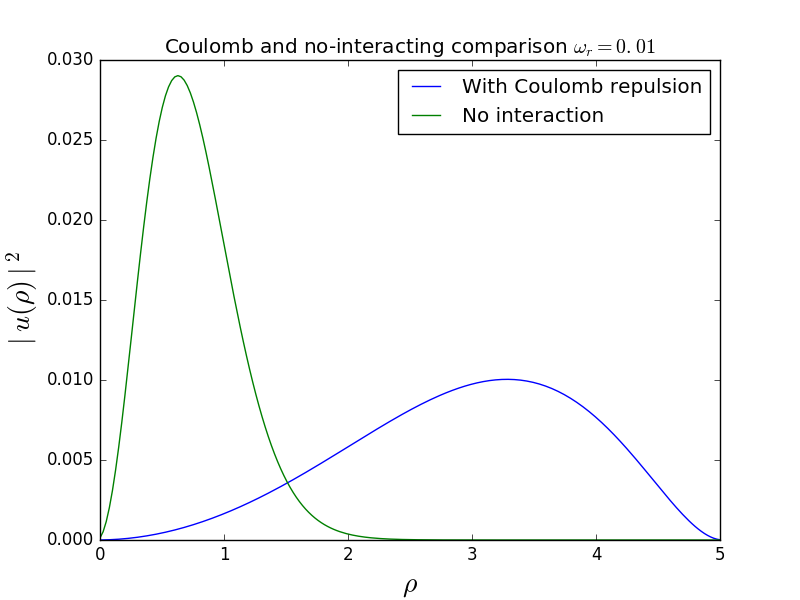
\includegraphics[width=0.9\textwidth]{../figures/interaction.png}
	\caption{Plot showing the difference between the ground state with and without Coulomb repulsion.}
\end{figure}

Knowing that the $|u(\rho)|^2$ describes the position of the particles, it is easy to see that the Coulomb repulsion results in the two particles being farther apart. This conclusion is quite intuitive when describing two repulsing particles. From \ref{fig:ConoCo} we observe this effect, as the "no interaction"-curve is sharper that with Coulomb repulsion.

\begin{figure}[ht]
	\label{fig:Co}
	\centering
	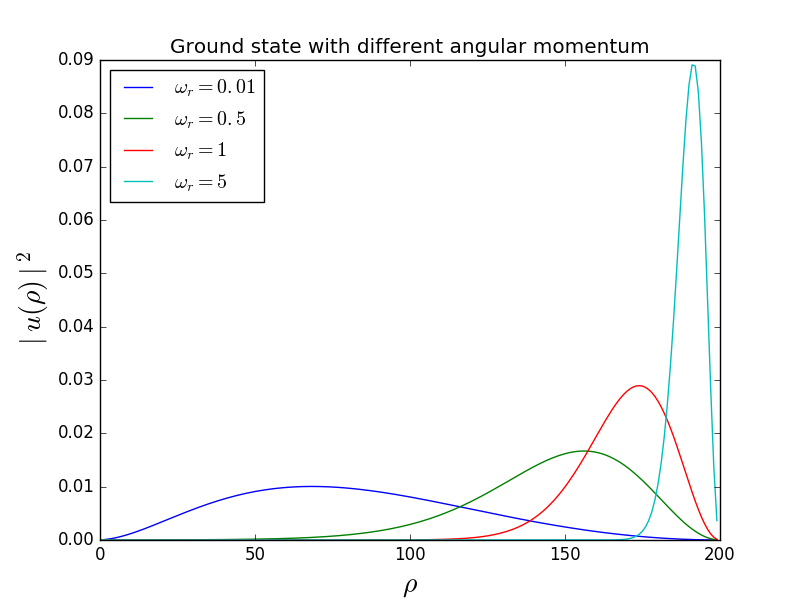
\includegraphics[width=0.9\textwidth]{../figures/omega.png}
	\caption{Plot of the ground state with Coulomb repulsion and varying angular momentum}
\end{figure}

In from figure \ref{fig:Co} we are looking at the case of Coulomb repulsion for varying frequencies $\omega_i$. Right away, we see that by increasing the oscillator frequency, we get sharper curves, meaning a more well defined position. This follows by the fact that $\omega_r$ determines the strength of the well resulting in the two electrons being forced closer together.

\section{Summary Remarks}
solving the Schrödinger equation as an eigenvalue problem. We have concluded that the behaviour of the two particles examined coincide well with that predicted from quantum mechanics. Furthermore, we have successfully implemented unit tests into our code, allowing us to locate errors in our code more efficiently. We have however not discussed the efficiency of our code, but can assume from what we learned in project 1 that a specialized algorithm for the given matrix would have resulted in a faster program. 

\begin{thebibliography}{9}

\bibitem{morten2}
	Hiorth-Jensen, M.,
	\emph{Project 2, Computational Physics I FYS3150/FYS4150},
	University of Oslo,
	2016.
	
\bibitem{abel}
	Abel, N.H.,
	Memoire sur le équations algébriques, ou l'on démontre l'impossibilité de la résolution de l'équation générale de cinquiéme degré,
	In Sylow, L. and Lie, S., 
	\emph{Æuvres Complètes de Niels Henrik Abel}, 2nd ed.,
	Grøndahl \& Søn, pp. 28-33,
	1881.

\end{thebibliography}

\begin{appendix}
\section{Laguerre Polynomials}
\label{app:laguerre}
Generally, the name Laguerre polynomials is used for solutions to 
\begin{equation}
x\frac{d^2y}{dx^2}+(\alpha+1-x)\frac{dy}{dx} + ny = 0.
\end{equation}
These polynomials, usually denoted, $L_0$, $L_1$, $L_2$ etc are a polynomial sequence which may be defined by the Rodriguez formula
\begin{equation}
L_n(x) = \frac{e^x}{n!}\frac{d^n}{dx^n}(e^{-x}x^n)=\frac{1}{n!}\left(\frac{d}{dx} -1 \right)x^n
\end{equation}
The first few Laguerre polynomials are shown in table \ref{tab:laguerre}.

\begin{table}[ht]
	\centering
	\caption{The first few Laguerre polynomials}
	\begin{tabular}{cl} \hline
	$n$ & $L_n(x)$  \\ \hline
	$0$ & $1$ \\
	$1$ & $-x+1$ \\
	$2$ & $\frac{1}{2}(x^2-4x+2)$ \\
	$3$ & $\frac{1}{6}(-x^3+9x^2-18x+6)$ \\
	$4$ & $\frac{1}{24}(x^4-16x^3+72x^2-96x+24$ \\
	$5$ & $\frac{1}{120}(-x^5+25x^4-200x^3+600x^2-600x+120) $ \\
	$6$ & $\frac{1}{720}(x^6-36x^5+450x^4-2400x^3+5400x^2-4320x+720)$ \\ \hline
	\end{tabular}
	\label{tab:laguerre}
\end{table}

\end{appendix}

\end{document}